% Generado por shared_vs_per_pedestrian.py
\begin{frame}[c]{Anexo: parámetros compartidos o por peatón (ECM 1)}
  \centering
  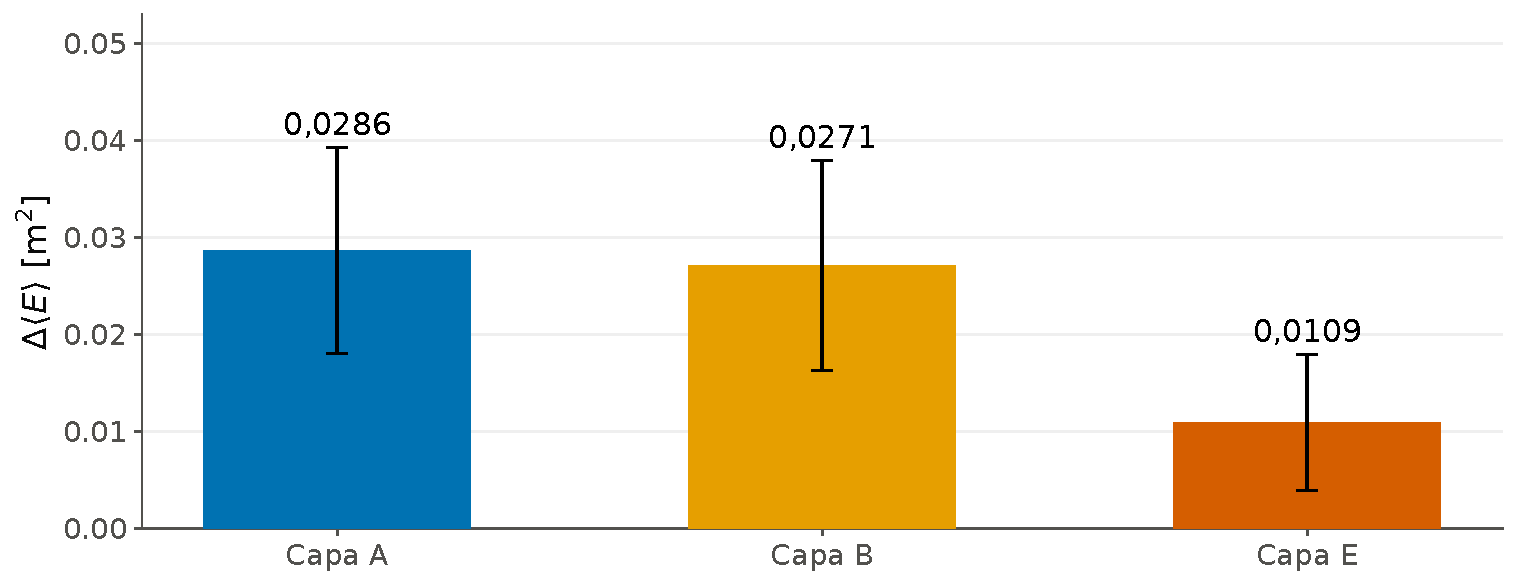
\includegraphics[width=\textwidth,height=3.4cm,keepaspectratio]{figuras/compartido-vs-por-peaton-ecm1.pdf}
  \par\vspace{1mm}
  {\footnotesize\renewcommand{\arraystretch}{1.15}
  \begin{tabular}{@{}lccc@{}}
  \hline Capa & $\langle E\rangle_{2p}$ (m$^2$) & $\langle E\rangle_{4p}$ (m$^2$) & Reducción \\ \hline
A & $0{,}4047$ & $0{,}3761$ & $7{,}1\,\%$ \\
B & $0{,}4022$ & $0{,}3751$ & $6{,}7\,\%$ \\
E & $0{,}3972$ & $0{,}3863$ & $2{,}8\,\%$ \\
  \hline
  \end{tabular}\par}
  \vspace{1mm}
  {\scriptsize 2p: un par compartido por evento; 4p: un par por peatón y por evento.\\
  Misma grilla amplia en ambos casos; los dos peatones se simulan juntos.\\
  $\Delta\langle E\rangle=\langle E\rangle_{2p}-\langle E\rangle_{4p}$; barras: $\pm$ error estándar entre eventos.\par}
\end{frame}
